\documentclass[modern]{aastex631}
\bibliographystyle{aasjournal}

%\turnoffedit

% \usepackage{fontspec}
% \usepackage[T1]{fontenc}
% \usepackage{newtxsf}
% \setmainfont{Fira Sans Book}[Scale=1.0]

\usepackage[caption=false]{subfig}
\usepackage{censor}
\usepackage{booktabs}
\usepackage{graphicx}
\usepackage{cancel}
\usepackage{float}
\usepackage[section]{placeins}
\usepackage{csquotes}
\graphicspath{{./figures/}}

%%%%%%%%%%%%%%%%%%%%%%%%%%%%%%%%%%%%%
%%%%% Some Useful Abbreviations %%%%%
%%%%%%%%%%%%%%%%%%%%%%%%%%%%%%%%%%%%%
\newcommand{\tess}{{\it TESS}}
\newcommand{\jwst}{{\it JWST}}
\newcommand{\kepler}{{\it Kepler}}
\newcommand{\ktwo}{{\it K2}}
\newcommand{\hst}{{\it HST}}
\newcommand{\msun}{$M_{\odot}$}
\newcommand{\rsun}{$R_{\odot}$}
\newcommand{\lsun}{$L_{\odot}$}
\newcommand{\re}{$R_{\oplus}$}
\newcommand{\me}{$M_{\oplus}$}
\newcommand{\rj}{$R_{\textrm{\scriptsize Jup}}$}
\newcommand{\mj}{$M_{\textrm{\scriptsize Jup}}$}
\newcommand{\ms}{m~s$^{-1}$}


\begin{document}
\shorttitle{Starspot contrast with TESS and K2}
\shortauthors{TBD}
\title{A systematic measurement on starspot contrast from TESS and K2
  bandpass differences}

\author{TBD}
\affiliation{University of Texas at Austin Department of Astronomy}

\author{TBD}
\affiliation{TBD}


\begin{abstract}

  Abstract goes here.

\end{abstract}

\keywords{Starspots (1572)}

\section{Introduction}\label{sec:intro}

The diminution of flux arising from occultations of the stellar disk contains information the relative sizes of the occulting bodies.  A commonsense exoplanet heuristic dictates that the relative transit depth $D$ equals the ratio of the bodies' projected areas ($R_p^2/R_\star^2$).  Additional correction factors account for limb darkening \citep{2002ApJ...580L.171M}.  Starspots on a stellar surface can exhibit spatial segregations
that yield \emph{unocculted starspots}: spots that are present on the surface but are not traversed during transits.  These unocculted starspots confound the mapping of transit depth to planet radius: a planet ``looks bigger'' than it really is if it blocks the brighter-on-average flux of the stellar disk \citep{2018AJ....156...91M}.  You cannot measure a planet radius without making some assumptions about the extent, contrast, and distribution of starspots.

The prevailing assumption within the exoplanet community has been that starspot covering fractions are small enough---as in Sunspots---to be ignored.  New theoretical models \citep{2018ApJ...853..122R} and observational evidence \citep{2016MNRAS.463.2494F} indicate that starspot covering fractions are large enough to bias transit depths beyond the level of precision of \kepler\ and \tess.  This so-called ``Transit Light Source Effect'' (TLSE) can bias derived exoplanet radii up to 17\% in the \tess\ bandpass, and can bias derived exoplanet \emph{densities} up to 50\%, since the radius error propagates into volume error with a factor of 3.  Therefore, TLSE threatens placement and interpretation of the exoplanet mass-radius relation science requirements of the \tess\ mission.  The interpretation of \jwst\ exoplanet transmission spectroscopy is also at risk \citep{2019AJ....157...11W}.



\begin{deluxetable}{chc}
  \tablecaption{Annotated bibliography for intro\label{table1}}
  \tablehead{
    \colhead{Reference} & \nocolhead{two} & \colhead{Key idea}
  }
  \startdata
  \citet{gullysantiago17} & - & LkCa~4 starspot spectral decomposition\\
  \citet{2015ApJ...807..174S} & - & Radius inflation from spots \\
  Strassmeier & - & Starspots review \\
  Rackham & - & TLSE \\
  \enddata
\end{deluxetable}



\section{Observations and Data Reduction}

All sources were observed by both the K2 \citep{howell14} and TESS \citep{2015JATIS...1a4003R} missions.

\subsection{Sample selection}
Our initial sample mirrors...

\subsection{TESS pipelines}


\subsection{Quality assurance checks}

\subsubsection{Handling data gaps}

\subsubsection{Handling multiple sectors}

\subsubsection{Quality flags}

\subsubsection{Outlier detection}

At first, the lightcurve program was falsely calculating many periods due to possible instrumental artifacts, flares, exoplanets, and background noise. To mitigate these outliers, we first tried using the \enquote{remove\_nans} and \enquote{remove\_outliers} methods. This helped, but still left many artifacts. Next, we decided to limit the period calculation to a maximum of 10 days and a minimum of 0.1 days.

After we finished extrapolating the data using the computer, we then developed several criteria by close inspection to further eliminate outliers. One such criterion was to discard any points that exceeded or subceeded 80\% of perfect correlation between the missions. and points with over a 7 days period. The first requirement was decided because anything that differs by more than 80\%, in our opinion, most certainly the result of data fluctuations. Similarly, we have to exclude any periods greater than 7 days due to TESS's time restraints. TESS only collected data for each object for around 22 days, so we set a 7-day maximum period to include 3 whole wavelengths.


\authorcomment1{Outliers attributable to instrumental artifacts}.

\authorcomment1{Outliers attributable to flares}.

\authorcomment2{Outliers attributable to exoplanets}.

\begin{figure}[!htb]
  \centering
  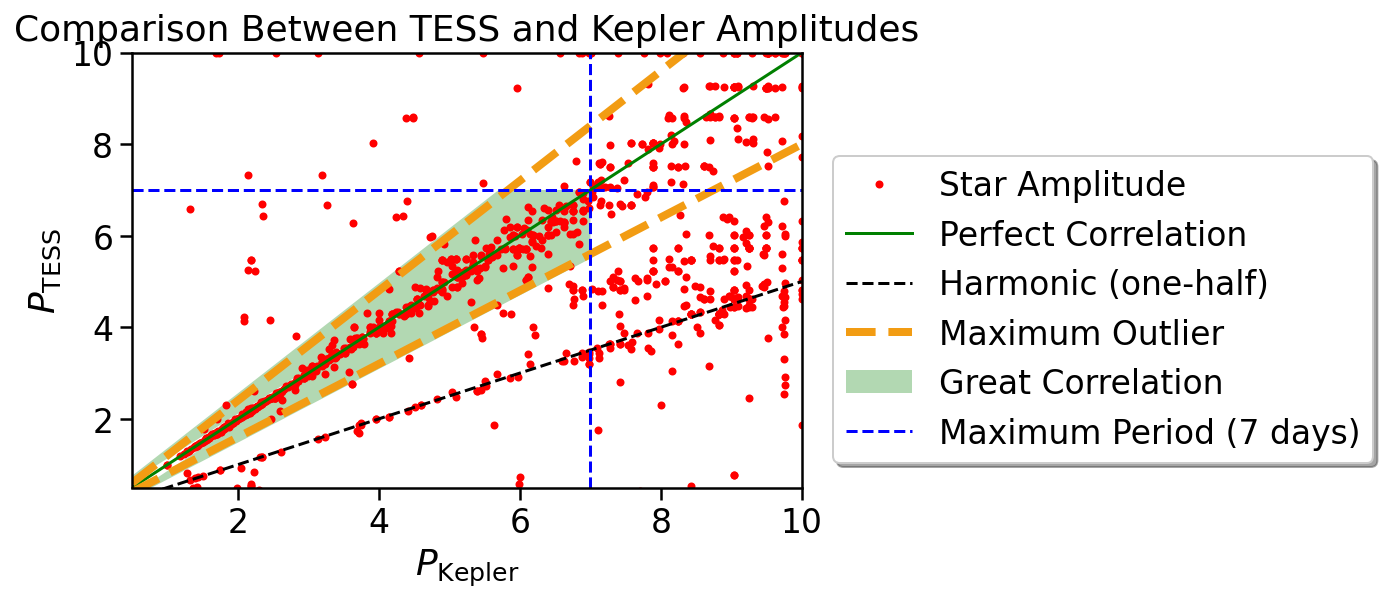
\includegraphics[scale=0.5]{Amplitude Comparison Mask.png}
  \caption{The mask showing how we determined which points were outliers.}
\end{figure}
\FloatBarrier

\section{Analysis}

Starspots emit light, which is often parameterized as \emph{spot contrast}, $c$, where $0$ means the spots are completely black compared to the bright photosphere, and $c=0.3$ means the spot has 30\% the flux per-unit-surface-area of the pristine photosphere.  Hypothetically, a contrast of unity would mean the starspot blends into ambient photosphere, its border vanishing entirely.  Spot contrast is wavelength dependent ($c_\lambda$). It has a spectrum of its own, starting close to zero in the blue/visible, and approaching perhaps 40\% in the near-IR; the exact prescription remains an active research area \cite{2005LRSP....2....8B}.  Zeeman splitting and other magnetic phenomena are secondary to the mere fact that starspots appear as cooler-than-average regions on the stellar surface.

Starspot flux can be parameterized by labeling the emission components with a characteristic temperatures
$T_\mathrm{spot}<T_\mathrm{phot}$.The spot and ambient photosphere spectra depend only on those temperatures: $S(T_\mathrm{spot})$ and $S(T_\mathrm{phot})$.  The wavelength-dependent spot contrast is then simply the ratio of the spot spectrum to the ambient photosphere spectrum:  $c_\lambda = \frac{S(T_\mathrm{spot})}{ S(T_\mathrm{phot})}$.

Figure \ref{fig:filtercurve} shows an illustration of wavelength dependent spot contrast for a hypothetical M0V star with $T_\mathrm{phot}=3800\;$K, and with $T_\mathrm{spot}=3300\;$K.  We employ \texttt{PHOENIX} synthetic spectral models \cite{2013A&A...553A...6H}, accessed at these temperatures.  The contrast ascends from near 0.01 at $\lambda=500\;$nm, to 0.15 at 1 $\mu$m.  By 2.3 $\mu$m, the contrast has peaked at 0.3.  The overlapping \kepler\ and \tess\ system throughputs overplotted on Figure \ref{fig:filtercurve} indicate that---on average---the starspot contrast is a lower number in the \kepler passband ($\lambda \sim 550\;$nm)  than for the redder \tess passband ($\lambda \sim 850\;$nm).  Starspots look blacker in \kepler\ and \ktwo\ than they do in \tess.  The understanding of wavelength dependent starspot contrast is not novel--- it has driven the design of precision radial velocity (PRV) spectrographs to the near-IR, where the deleterious effect of starspots on RV jitter is lessened.  The key innovation of this proposal stems from the vast number of sources with existing \ktwo\ data that \tess\ will observe in Cycle 4.  This proposal aims to quantify precisely the starspot contrast differences between the \tess\ and \kepler\ wavelength bands.  We re-iterate that the extent to which nature produces starspot spectra resembling the prescription in Figure \ref{fig:filtercurve} remains an unknown, and is the main thrust of the proposed work effort.

System-throughput-weighted contrast spectra can be integrated over the illustrated filter curves to yield precision estimates for contrasts in the two passbands.  For this M0V example, we obtain $c_{\ktwo}\sim0.025$ and $c_{\tess}\sim0.1$.  Starspots appear about four times darker in \kepler\ and \ktwo\ than they do in \tess.  We define the ratio of starspot contrasts of \tess\ compared to \kepler\ as $\mathcal{R}\equiv \frac{c_{\tess}}{c_{\ktwo}}$.  This proposal will systematically measure $\mathcal{R}$ for a vast number of stars observed by both missions.

\noindent \textbf{Spot-induced modulation amplitudes depend on contrast.}

Rotationally-modulated lightcurves exhibit semi-sinusoidal undulations as starspots (or spot groups) enter and exit the projected stellar disk.  The most-spotted projected hemisphere is directed towards the observer at the moment of the lightcurve minimum, and the least-spotted projected hemisphere at lightcurve maximum.  The amplitude of the lightcurve, therefore, is approximately the difference in starspot coverage fractions $\Delta f_{spot} \equiv f_{max}-f_{min}$ between the most-and-least spotted projected hemispheres, weighted by the spot contrast: $ A_\lambda = \Delta f_{spot} \cdot (1-c_\lambda)$.  Therefore the ratio of \tess\ to \kepler\ amplitudes yields a constraint independent of the actual spot coverage fraction:

$$ \frac{A_{TESS}}{A_{Kepler}} = \cancel{\frac{\Delta f_{spot}}{\Delta f_{spot}}} \cdot \frac{1-c_{TESS}}{1-c_{Kepler}} $$

The notation is cumbersome, but the takeaway is clear: we can quantify spot contrast ratio knowing only the amplitudes of \ktwo\ and \tess\ spot-modulated lightcurves.  This equation is approximate, and in practice our team will derive $\mathcal{R}= \frac{c_{\tess}}{c_{\ktwo}}$ with Monte Carlo methods to take into account the uncertainty of the amplitude determination and subtle starspot self-dilution effects.
\newline

\noindent \textbf{Head-to-head comparison of K2 and TESS amplitudes in the ecliptic fields}



The main two factors that affect spot-modulation lightcurve amplitudes are effective temperature (\emph{i.e.} mass), and rotation period (\emph{i.e.} stellar activity/magnetic fields) \cite{2014ApJS..211...24M}.  Other important-albeit-unknown factors like stellar inclination angle and multiplicity \emph{cancel out} when we compare the same stars head-to-head.  We, therefore, construct a plot of amplitude versus period, grouped by spectral type bins.  The \tess\ and \ktwo\ samples should look identical in these plots, but the locus of \tess\ sources resting systematically below the \ktwo\ sample, as in Figure \ref{fig:expected}.


The fact that observations are not contemporaneous adds some \emph{cosmic variance}: stars wander into and out-of their respective stellar minimum and maximum activity cycles, altering their amplitudes in 2021 compared to say 2018. So it is therefore impossible to assign a starspot contrast ratio $\mathcal{R}$ for any individual star.  Instead, we propose to measure the mean value of \emph{ensembles} of thousands of stars, again grouped by sources of similar properties.  On average stars will enter and exit stellar activity cycles in equal measure injecting per-star variance, but keeping the subsample mean $\mathcal{R}$ the same.

\subsection{Period measurement}


\subsubsection{Amplitude measurements}


% Helpful resource on how to insert and align images
% https://www.overleaf.com/learn/latex/Inserting_Images
\begin{figure}[!htb]
  \centering
  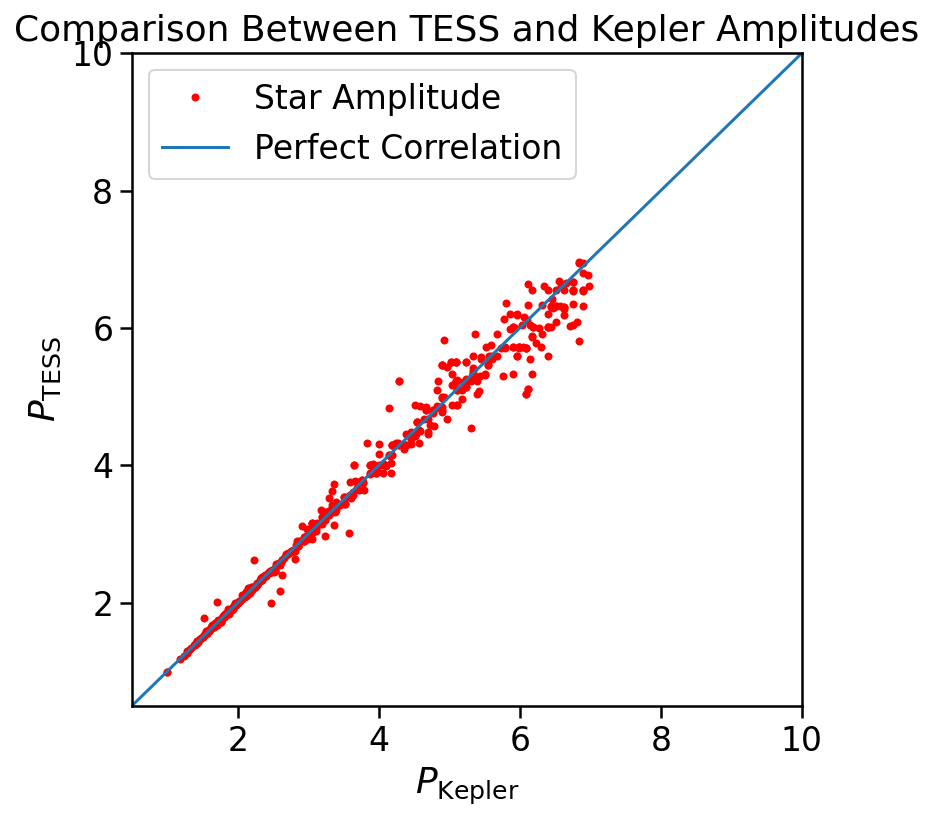
\includegraphics[scale=0.5]{Comparison Between TESS and Kepler Amplitudes.png}
  \caption{Relationship between the calculated amplitudes of TESS and Kepler and how close they are to unity.}
\end{figure}
\FloatBarrier


\section{Results}

\subsection{Amplitude versus rotation period for bins in $T_{\mathrm{eff}}$}

\subsection{TESS-to-K2 amplitude ratio as a function of $T_{\mathrm{eff}}$}

As seen in the figure below, the Kepler data are, on average, around 70 times larger than TESS's.

\begin{figure}[!htb]
  \centering
  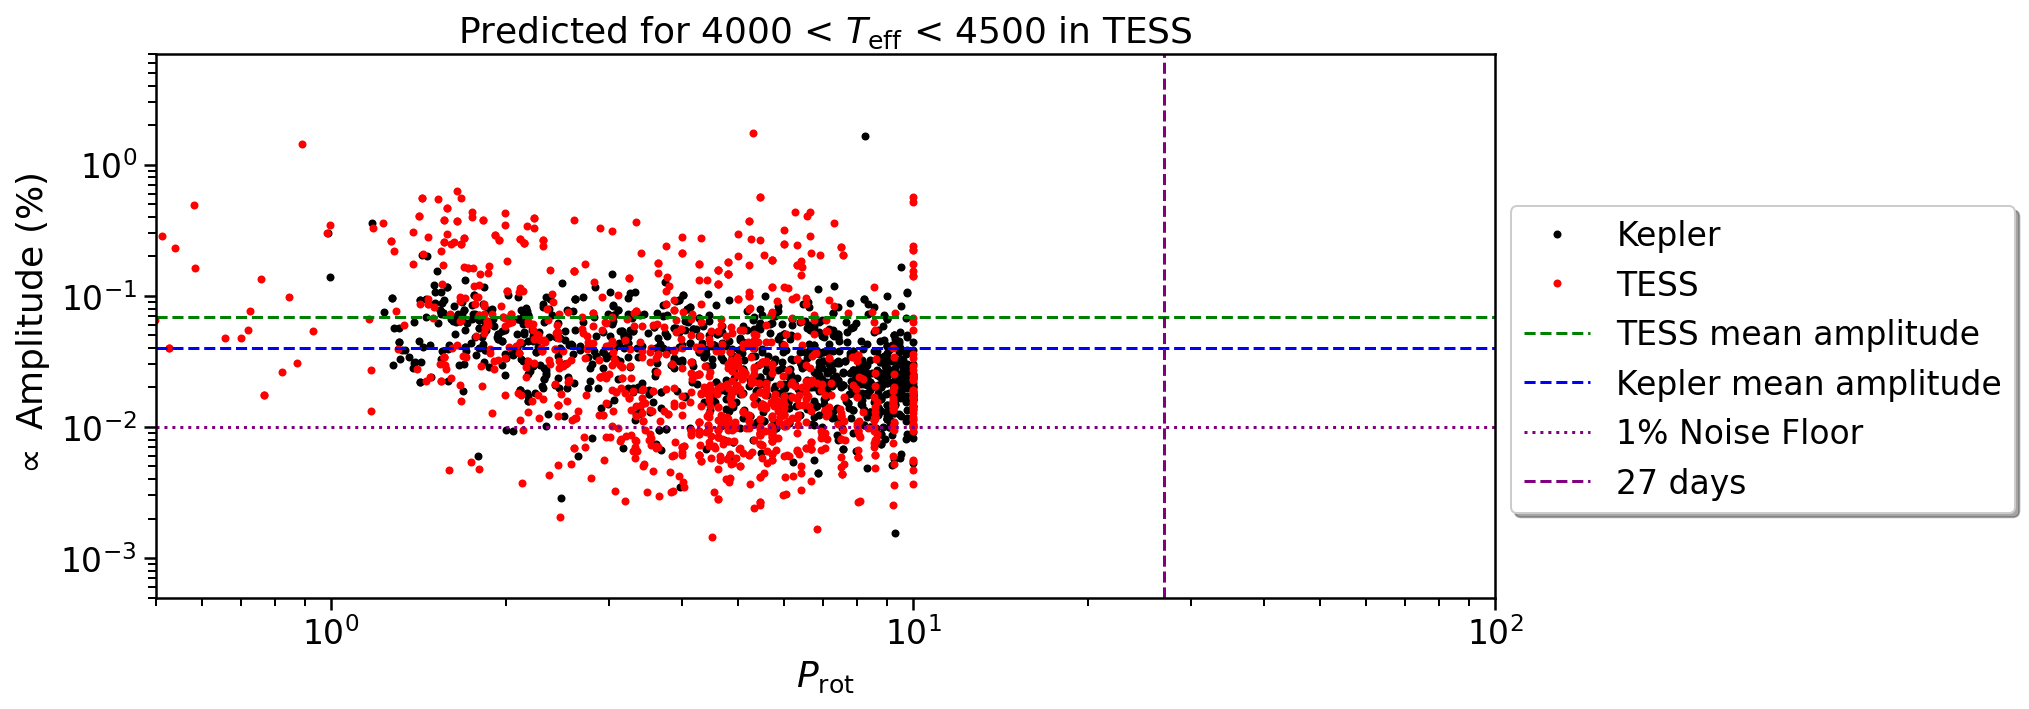
\includegraphics[scale=0.42]{Amplitude vs. Rotation for Kepler and TESS.png}
  \caption{Effect size for starspot contrast as seen in modulation amplitude versus period ($P_{\mathrm{rot}}$ [days]). The black points are the locus of spotted stars in the Kepler as measured by for late K dwarfs. The red points are the same stars, but measured with the TESS mission. The blue and green dashed lines represents the average amplitudes for all plotted stars for both Kepler and TESS, approximately 9350 and 130, respectively.}
\end{figure}
\FloatBarrier

\subsection{Converting amplitude ratio to $T_{\mathrm{spot}}$}

\subsection{Inferred $T_{\mathrm{spot}}$ versus $T_{\mathrm{eff}}$}


\section{Discussion}

\subsection{Comparison to other studies}
\citet{2016MNRAS.463.2494F} targeted 304 Pleiades sources with LAMOST and found the $T_{\mathrm{spot}}$ scales with $T_{\mathrm{eff}}$ with figure.

\subsection{Assessing the spots versus faculae}
Up to the this point, we have assumed that all flux variations arise from dark spots on the surface of the star. Stars can just as likely have bright patches that cause flux perturbations to their light curves. Here we assess the consequences of assuming faculae instead of spots.

\section{Conclusions}

\begin{acknowledgements}
  This paper includes data collected by the TESS mission. Funding for the TESS mission is provided by the NASA's Science Mission Directorate.

  The authors acknowledge the Texas Advanced Computing Center (TACC, \url{http://www.tacc.utexas.edu}) at The University of Texas at Austin for providing HPC resources that have contributed to the research results reported within this paper.
\end{acknowledgements}

\clearpage


\facilities{Gemini:South, TESS, ASAS, Gaia}

\software{
  pandas \citep{mckinney10, reback2020pandas},
  emcee \citep{foreman13},
  matplotlib \citep{hunter07},
  astroplan \citep{astroplan2018},
  astropy \citep{exoplanet:astropy13,exoplanet:astropy18},
  exoplanet \citep{exoplanet:exoplanet},
  numpy \citep{harris2020array},
  scipy \citep{jones01},
  ipython \citep{perez07},
  bokeh \citep{bokehcite},
  seaborn \citep{waskom14}}
%pytorch \citep{NEURIPS2019_9015}} % No pytorch yet!


\bibliography{ms}


\clearpage

\appendix
\restartappendixnumbering

\section{Optional appendix} \label{appendix:tools}

Place optional content here.
\end{document}